\PassOptionsToPackage{unicode}{hyperref}
\documentclass[aspectratio=43, professionalfonts, 9pt]{beamer}

\usefonttheme[onlymath]{serif}
\usetheme[showtotalframes]{tudo}

\ifluatex
  \usepackage{polyglossia}
  \setmainlanguage{german}
\else
  \ifxetex
    \usepackage{polyglossia}
    \setmainlanguage{german}
  \else
    \usepackage[german]{babel}
  \fi
\fi


% Mathematik
\usepackage{amsmath}
\usepackage{amssymb}
\usepackage{mathtools}
\usepackage{cancel}

\usepackage{hyperref}
\usepackage{bookmark}
\usepackage{animate}
\usepackage[autostyle]{csquotes}

\newcommand{\bunderbrace}[2]{
  \begin{array}[t]{@{}c@{}}
  \underbrace{#1}\\
  #2
  \end{array}
}


%%%%%%%%%%%%%%%%%%%%%%%%%%%%%%%%%%%%%%%%%%%%%%%%%%%%%%%%%%%%%%%%%%%%%%%%%%%%%%%%
%%%%%-------------Hier Titel/Autor/Grafik/Lehrstuhl eintragen--------------%%%%%
%%%%%%%%%%%%%%%%%%%%%%%%%%%%%%%%%%%%%%%%%%%%%%%%%%%%%%%%%%%%%%%%%%%%%%%%%%%%%%%%

%Titel:
\title{Analyse von Polymerkonfigurationen mit Neuronalen Netzen}
%Autor
\author[C.~Vorsmann]{Clemens Vorsmann}
%Lehrstuhl/Fakultät
\institute[Theoretische Physik I]{AG Kierfeld \\  Fakultät Physik}
%Titelgrafik
%\titlegraphic{\includegraphics[width=0.7\textwidth]{images/tudo-title-2.jpg}}


\begin{document}

\maketitle

w\section{Einleitung}

\begin{frame}
\frametitle{Inhaltsübersicht}
\tableofcontents%[pausesections]
\end{frame}


%\section{Einleitung}
\begin{frame}
  \frametitle{Worum gehts? Motivation} %die mesten horen wahrscheinlch floquet theorie zum ersten mal, deshalb nochmal etwas genauer, worum es geht
  \begin{itemize}
    \item 
\end{frame}

\section{Simulation}
\subsection{Polymermodell}

\begin{frame}
       \begin{tabular}{cl}
         \begin{tabular}{c}
           \includegraphics[width=0.5\textwidth]{Plots/rubinstein.png}
           \end{tabular}
           & \begin{tabular}{l}
             \parbox{0.5\linewidth}{
             \begin{itemize}
               \setlength\itemsep{1em}
               \item Monomere bestehen aus \textit{beads}\\ und \textit{bonds} \\
               \item N Monomere \\(Polymerisationsgrad)
               \item Bondvektoren $\vec{b}_i$ mit Länge $b$ \\
             \end{itemize}

             }
             \end{tabular}  \\
         \end{tabular}
         \begin{tiny}Quelle: Rubinstein, Michael and Colby, Ralph H. - Polymer Physics\\
         \end{tiny}
         \begin{itemize}
           \item $\Theta_{ij}$ ist Winkel zwischen $\vec{b}_i$ und $\vec{b}_j$ \\
           \item End-zu-End-Abstand $\vec{R}=\sum_{i=0}^{N-1} \vec{b}_i$
         \end{itemize}
\end{frame}

%\begin{frame}
%  \frametitle{wichtige Messgrößen}
%  \begin{block}{Definitionen}
%     \begin{itemize}
%       \item $\langle O \rangle = \frac{1}{Z} \sum_{i} O \text{e}^{-\beta E_i}$
%       \item $Z = \sum_i \text{e}^{-\beta E_i}$
%       \item $\langle R^2 \rangle = b^2 \sum_{i=0}^{N-1} \sum_{j=0}^{N-1} \langle \text{cos} \, \Theta_{ij} \rangle$
%       \item $\vec{t}_i = \frac{\vec{b}_i}{b}$
%       \item $\vec{t}_i \cdot \vec{t}_j = \text{cos} \, \Theta_{ij}  = \text{exp}{\left(- \frac{\lvert i - j \rvert}{ L_{\mathrm{p} }} \right)} $
%     \end{itemize}
%  \end{block}
%\end{frame}
\begin{frame}
   \frametitle{Wormlike-Chain (WLC)}
   \begin{block}{Definition über die Biegeenergie}
     \begin{itemize}
       \item $\vec{t}_i = \frac{\vec{b}_i}{b}$
       \item $\kappa = E \cdot I \sim E \cdot a^4$
       \item $E_{\text{bond}} = \frac{\kappa}{b} (1 - \text{cos}\,\Theta_{i-1,i})$
       \item $E_{\mathrm{Biege}}^{\mathrm{Ges}} = \frac{\kappa}{2b}\,\sum_{i=1}^{N-1} \left( \vec{t}_{i-1} - \vec{t}_{i}  \right)^2$
       \item $ \langle \vec{t}_i \cdot \vec{t}_j \rangle = \langle \text{cos} \, \Theta_{ij} \rangle  = \text{exp}{\left(- \frac{\lvert i - j \rvert}{ L_{\mathrm{p} }} \right)} $
     \end{itemize}
   \end{block}
   \begin{block}{Persistenzlänge der WLC}
     \begin{itemize}
       \item $L_{\mathrm{p}} = -\frac{b}{\coth \frac{\kappa}{b\,\mathrm{k_B\,T}} - \frac{b}{\kappa}\,\mathrm{k_B} \, T }$
     \end{itemize}
  \end{block}
\end{frame}

\begin{frame}
  \frametitle{Klassifizierung nach Flexibilität}
  \begin{figure}
    \centering
    \includegraphics[width=\textwidth]{Plots/regime.png}
    \caption{Quelle: Dissertation Tobias Kampmann}
    \label{fig:regime}
  \end{figure}
\end{frame}

\subsection{Monte-Carlo Simulation}

\begin{frame}
  \frametitle{Markow-Sampling}
  \begin{itemize}
    \item Berechnung von Erwartungswerten, mittels Zufallsprozessen
    \item Sampling vereinfacht Erwartungswert zu $\langle O \rangle = \frac{1}{n} \sum_{i=0}^n O(i)$
    \item Dafür zwei Bedingungen: \\
          \begin{enumerate}
            \item Detailliertes Gleichgewicht
            \item Ergodizität
          \end{enumerate}
  \end{itemize}
  \begin{block}{Detailliertes Gleichgewicht}
    \begin{itemize}
      \item $\frac{m_{ij}}{m_{ji}} = \frac{p_j}{p_i}$
    \end{itemize}
  \end{block}
\end{frame}

\begin{frame}
  \frametitle{Metropolis Algorithmus}
  \begin{itemize}
    \item Vorschlagsmoves mit Vorschlagswahrscheinlichkeit $V_{ij}$
    und Akzeptanzwahrscheinlichkeit $A_{ij}$
    \item $m_{ij} = V_{ij}A_{ij}$
  \end{itemize}
  \begin{block}{Metropolis-Filter}
    \begin{itemize}
      \item $A_{ij} = \text{min}( 1, \frac{p_i}{p_j})$
      \item $V_{ij} = V_{ji}$
    \end{itemize}
  \end{block}
  \begin{itemize}
    \item $p_i \propto \text{exp}(-\beta E_i)$
  \end{itemize}
\end{frame}

\begin{frame}
  \frametitle{Monte-Carlo-Moves}
  \begin{enumerate}
    \item Wähle zufälligen Bead
    \item Drehe zugehörigen Bondvektor, um $\Delta\Theta$
    \item $\Delta E = E_{\text{alt}}-E_{\text{neu}}$
    \item Fallunterscheidung:\\
         \setbeamertemplate{enumerate items}[square]
         \begin{enumerate}
           \item $\Delta E \geq 0$: akzeptiere Vorschlag
           \item $\Delta E < 0$: akzeptiere mit Wahrscheinlichkeit
                 $\text{exp}(\beta \Delta E)$
         \end{enumerate}
  \end{enumerate}
\end{frame}

\begin{frame}
\begin{minipage}[t]{0.5\textwidth}
\includegraphics[width=\textwidth]{Plots/Energie.pdf}
\end{minipage}%
\hfill%
\begin{minipage}{0.5\textwidth}
\begin{itemize}
  \item Parameter $N=100$, $b=1$, $\kappa=100$, $\beta = 1$
  \item zufällige Anfangskonfiguration
  \item Äquilibrierungszeit von ca. $10^3$ Durchläufen
  \item Äquipartitionstheorem: $\langle E \rangle = 1\,\text{k}_{\text{B}}T$
        pro Bond
\end{itemize} \vspace{2.5cm}
\end{minipage}

\end{frame}


\begin{frame}
  \frametitle{Tangentenkorrelationen}
  \begin{itemize}
    \item $L_{\mathrm{p}} = -\frac{b}{\coth \frac{\kappa}{b\,\mathrm{k_B\,T}} - \frac{b}{\kappa}\,\mathrm{k_B} \, T } \approx 99.5 $ \\
    \item $\langle \vec{t}_i \cdot \vec{t}_{i+j} \rangle = \sum_{i=0}^{N-1-j} \vec{t}_i \cdot \vec{t}_{i+j}$
  \end{itemize}
  \begin{figure}
    \centering
    \includegraphics[width=0.6\textwidth]{Plots/korr13.pdf}
    \label{fig:tangkorr}
  \end{figure}
\end{frame}

\begin{frame}
  \frametitle{Erzeugung von Messwerten}
  \begin{minipage}{0.4\textwidth}
  \begin{itemize}
    \item künstliches Neuronales Netz soll aus Polymerkonfiguration
          dessen Biegesteifigkeit bestimmen
    \item $N=100$, $b=1$, $\beta = 1$
    \item $10 \leq \kappa \leq 20$
    \item Momentaufnahme: Winkel $\Theta_{i-1,i}$, $\kappa$
  \end{itemize}
  \end{minipage}%
  \hfill%
  \begin{minipage}{0.4\textwidth}
  \includegraphics[width=\textwidth]{Plots/polymer1.pdf}
  \end{minipage}\\
  \begin{minipage}{0.4\textwidth}
    \begin{figure}
     \includegraphics[width=\textwidth]{Plots/pixel-reduction.png}
     \caption{\url{https://link.aps.org/doi/10.1103/PhysRevE.48.R1642}}
    \end{figure}
  \end{minipage}%
  \hfill%
  \begin{minipage}{0.4\textwidth}
    \begin{figure}
    \includegraphics[width=\textwidth]{Plots/fluorescene-winkel.png}
    \end{figure}
  \end{minipage}
\end{frame}

\begin{frame}
  \frametitle{Beispielkonfigurationen}
  \begin{figure}
    \centering
    \includegraphics[width=\textwidth]{Plots/blurred33.png}
    \label{fig:bsp}
  \end{figure}
\end{frame}

\section{künstliche Neuronale Netze}
\subsection{Multilayer Perceptron}

\begin{frame}
  \frametitle{Grundlagen}
  \begin{minipage}{0.5\textwidth}
   \begin{itemize}
     \item Eingabevektor $\vec{x}_l$
     \item Gewichtmatrix $\mathbf{W}^{\left( l \right)}$
     \item Aktivierungsfunktion $g^{\left( l \right)}$
     \item maAusgabevektor $\vec{y}^{(l)}$
   \end{itemize}
  \end{minipage}%
  \hfill%
  \begin{minipage}{0.5\textwidth}
    \begin{figure}
      \centering
      \includegraphics[width=\textwidth]{Plots/neuralnetworkhaykin.png}
      \caption{Quelle: Haykin, S.S., Neural Networks: A Comprehensive Foundation}
    \end{figure}
  \end{minipage}
\end{frame}

\begin{frame}
  \frametitle{mathematische Formulierung}
  \begin{block}{Definitionen}
    \begin{itemize}
      \item $\vec{y}^{\left( l \right)} = g^{\left( l \right)}
              \left( \bunderbrace{ \mathbf{W}^{\left( l \right)}
              \vec{x}^{\left( l \right)} + \vec{b}^{\left( l \right)}}
              {\coloneqq \vec{v}^{\left(l\right)} }  \right)$
      \item $g^{(l)}(\vec{x}^{(l)}) = g(\vec{x}^{(l)}) = ReLU \left( x \right) = \max \left ( 0,x \right)$
    \end{itemize}
  \end{block}
\end{frame}


\begin{frame}
  \frametitle{verschiedene Aktivierungsfunktionen}
  \begin{figure}
    \centering
    \includegraphics[width=0.8\textwidth]{Plots/Aktivierungsfunktionen.pdf}
  \end{figure}
\end{frame}

\subsection{Lernen und Fehlerrückführung}
\begin{frame}
  \frametitle{Ablauf des Lernalgorithmus}
  \begin{enumerate}
    \item Hinführung: Vorhersagewert $\vec{y}^{(l)}$, richtiger Wert $\vec{d}^{(l)}$
    \item Mean-squared-error (MSE) $\epsilon(n)$
    \item Fehlerrückführung: $\Delta w_{ij}^{\left( l \right)}\left(n\right)$
  \end{enumerate}
   \begin{block}{MSE, Gradientenabstiegsverfahren}
      \begin{itemize}
        \item $\epsilon \left ( n \right) = \frac{1}{2} \left( \vec{d}^{\left( l \right)}\left( n \right) -  \vec{y}^{\left( l \right)}\left( n \right)\right)^2$
        \item $\Delta w_{ij}^{\left( l \right)}\left(n\right) = - \eta \, \frac{\partial \epsilon\left(n\right)}{\partial w_{ij}^{\left( l \right)}\left(n\right) }$
      \end{itemize}
   \end{block}
\end{frame}

\begin{frame}
   \frametitle{Anpassung des Gradientenabstiegsverfahrens}
   \begin{itemize}
     \item kleine Lernrate: langsame Konvergenz
     \item große Lernrate: \enquote{Zig-Zagging}
     \item Impulskonstante $\alpha$
   \end{itemize}
   \begin{block}{Gradientenabstiegsverfahren mit Impulsterm}
      \begin{itemize}
        \item $\Delta w_{ij}^{\left( l \right)}\left(n\right) = - \eta \, \frac{\partial \epsilon\left(n\right)}{\partial w_{ij}^{\left( l \right)}\left(n\right) } + \alpha \Delta w_{ij}^{\left( l \right)}\left(n-1\right) $
      \end{itemize}
   \end{block}
\end{frame}

\begin{frame}
  \frametitle{Lern-Modi}
  \begin{itemize}
    \item Stochastic-Mode
    \item Batch-Mode
    \item Mini-Batch-Mode
  \end{itemize}
  \begin{block}{Gewichtsanpassung im Mini-Batch-Mode}
    \begin{itemize}
      \item $\Delta w_{ij}^{\left( l \right)}\left(n + 1\right) = \alpha \, w_{ij}^{\left( l \right)}\left(n + 1\right)
         + \eta \, \delta_j^{\left( l \right)}\left(n \right) \, y_i^{\left( l-1 \right)}\left(n \right)$
      \item $\delta_{j}^{\left( l \right)}\left(n \right) =
            \begin{dcases*}
              \left( d_j \left( n \right) - y_j^{\left( L \right)} \left(n \right) \right) \, g'\left( v_j^{\left(L \right)}\right)
              ,& \small{$j$-tes Perzeptron in Ausgabeschicht $L$}\\
              g'\left( v_j^{\left(l \right)}\right) \sum_{k} \delta_k^{\left(l+1\right)}\left(n\right) w_{kj}^{\left(l+1\right)}\left(n\right)
              ,& \small{$j$-tes Neuron in versteckter Schicht $l$}
            \end{dcases*}$
    \end{itemize}
  \end{block}

\end{frame}


\subsection{Trainieren des Neuronalen Netzes}

\begin{frame}
  \frametitle{Aufbau eines einfachen Modells}
  \begin{minipage}{0.5\textwidth}
    \begin{figure}
      \centering
      \includegraphics[width=\textwidth]{Plots/model_plot.pdf}
    \end{figure}
  \end{minipage}%
  \hfill%
  \begin{minipage}{0.5\textwidth}
    \begin{enumerate}
      \item input layer - 99 Neuronen
      \item hidden layer - 20 Neuronen
      \item hidden layer - 10 Neuronen
      \item output layer - 1 Neuron
    \end{enumerate}
  \end{minipage}
\end{frame}

\begin{frame}
  \frametitle{Overfitting und Early Stopping}
  \begin{figure}
    \centering
    \includegraphics[width=0.8\textwidth]{Plots/MSE.pdf}
  \end{figure}
\end{frame}

\begin{frame}
  \frametitle{Early Stopping - aber wann?}
  \begin{figure}
    \centering
    \includegraphics[width=0.8\textwidth]{Plots/MSE150k.pdf}
  \end{figure}
\end{frame}

\begin{frame}
  \frametitle{Graphische Veranschaulichung zur Validierung}
  \begin{figure}
    \centering
    \includegraphics[width=0.8\textwidth]{Plots/mlp_test_new.pdf}
  \end{figure}
\end{frame}

\begin{frame}
  \frametitle{Hyperparameteroptimierung im Vergleich}
  \begin{minipage}{0.5\textwidth}
    \begin{figure}
      \centering
      \includegraphics[width=\textwidth]{Plots/MSEOpt.pdf}
    \end{figure}
  \end{minipage}%
  \hfill%
  \begin{minipage}{0.5\textwidth}
      \begin{itemize}
        \item Konfigurationsraum \\
        \begin{enumerate}
          \item Anzahl Neuronen in den versteckten Schichten
          \item Dropoutlayer zwischen den versteckten Schichten
        \end{enumerate}
        \item Tree-Structured Parzen Estimator (TPE), jeweils 1000 Epochen
      \end{itemize}
  \end{minipage}
  \begin{minipage}{\textwidth}
     \begin{enumerate}
       \item input layer - 99 Neuronen
       \item hidden layer - 20 Neuronen
       \item dropout layer - 33.8 \%
       \item hidden layer - 8 Neuronen
       \item output layer - 1 Neuron
     \end{enumerate}
  \end{minipage}

\end{frame}

\begin{frame}
  \frametitle{Einfluss mehrerer Aufnahmen}
  \begin{minipage}{0.7\textwidth}
    \begin{figure}
      \centering
      \includegraphics[width=\textwidth]{Plots/multiple.pdf}
    \end{figure}
  \end{minipage}%
  \hfill%
  \begin{minipage}{0.3\textwidth}
    \begin{figure}
      \centering
      \includegraphics[width=\textwidth]{Plots/f-aktin.png}
      \caption{Quelle: \url{https://link.aps.org/doi/10.1103/PhysRevE.48.R1642}}
    \end{figure}
  \end{minipage}
\end{frame}

%\begin{frame}
%       \begin{tabular}{cl}
%         \begin{tabular}{c}
%           \includegraphics[width=0.5\textwidth]{Plots/Aktivierungsfunktionen.pdf}
%           \end{tabular}
%           & \begin{tabular}{l}
%             \parbox{0.5\linewidth}{%  change the parbox width as appropiate
%             $\text{ReLU}(x) = \text{max}(0,x)$
%                                    }
%             \end{tabular}  \\
%         \end{tabular}
%\end{frame}

\section{Fazit und Ausblick}

\begin{frame}
  \frametitle{Ausblick}
  \begin{itemize}
    \item Monte-Carlo Daten stimmen mit Theorie überein
    \item Multilayer-Perceptron eignet sich, um aus Winkelverteilung
    die Biegesteifigkeit zu bestimmen
    \item Hyperparameteroptimierung aufwendig, hier nicht erfolgreich
    \item Spare Bildverarbeitungsschritt mit Convolutional Neural Network
    \item Problem: Bild ist lediglich 2d-Projektion
  \end{itemize}
\end{frame}



\end{document}
